\section{Introduction}

\para{Targeted Problem.}
Long-context problem is a core bottleneck for coding LLMs: realistic workflows include repository-level code snippets, long test logs, and multiple tool observations that easily exceed typical context budgets. When the full context is not provided, models can fail due to missing critical information. When the full context is provided, inference becomes costly, and the model may still be unreliable because attention is spread across redundant or noisy text; empirically, accuracy can degrade when relevant evidence appears in the middle of long contexts \cite{liu2023lost,hsieh2024ruler,bai2023longbench_arxiv}. Therefore, effective long-context handling is crucial for coding LLMs \cite{vaswani2017attention,dao2022flashattention}.

\para{Existing Methods.}
State-of-the-art long-context strategies for coding LLMs mainly fall into three categories. First, retrieval-based approaches select small subsets of repository context (files, functions, or chunks) to fit within a budget \cite{lewis2020rag,karpukhin2020dpr,robertson2009bm25}. Second, pruning-based methods attempt to discard irrelevant lines in logs/diffs or compress context while preserving salient parts; agentic systems such as SWE-agent operationalize iterative retrieval and tool interaction for software tasks \cite{yang2024sweagent,yao2022react,schick2023toolformer}. Third, summarization-based methods replace long observations with model-generated summaries or compressed prompts \cite{jiang2023llmlingua}. While effective in many settings, each category has its own shortcomings (e.g., missing relevant evidence, over-pruning, or unfaithful summaries), so robust long-context handling for coding LLMs remains an open problem \cite{liu2023lost,hsieh2024ruler}.

\para{Research Gap.}
Recently, a new context compression technique, which we refer to as \emph{optical compression}, has emerged. The key idea is to turn long text into images and feed them to a vision-capable LLM, potentially reducing the number of text tokens needed while still conveying the same information. This approach has shown promise in document-oriented settings \cite{kim2021donut,lee2022pix2struct,openai2023gpt4v_systemcard}, but its utility for coding LLMs is unclear. On the one hand, optical compression could make it cheaper to pass long tool outputs (e.g., logs, stack traces, diffs, and multi-file code) and may mitigate long-context brittleness by preserving more raw evidence \cite{liu2023lost}. On the other hand, image-based encoding can introduce new error modes (e.g., character-level corruption or missed symbols) which can be particularly harmful for code \cite{shi2023gpt4v_ocr}. Overall, there is limited systematic evidence on whether off-the-shelf coding LLMs benefit from optical compression, and how such encoding affects the cost--fidelity--performance tradeoff \cite{wei2025deepseekocr,feng2026agentocr}.

\para{Research Question.}
To this end, we focus on a question: in an agentic coding setting with no post-training, can a vision-capable LLM read source code from rendered images as effectively as from plain text, and what are the cost and behavioral implications?

\begin{figure}[t]
  \centering
  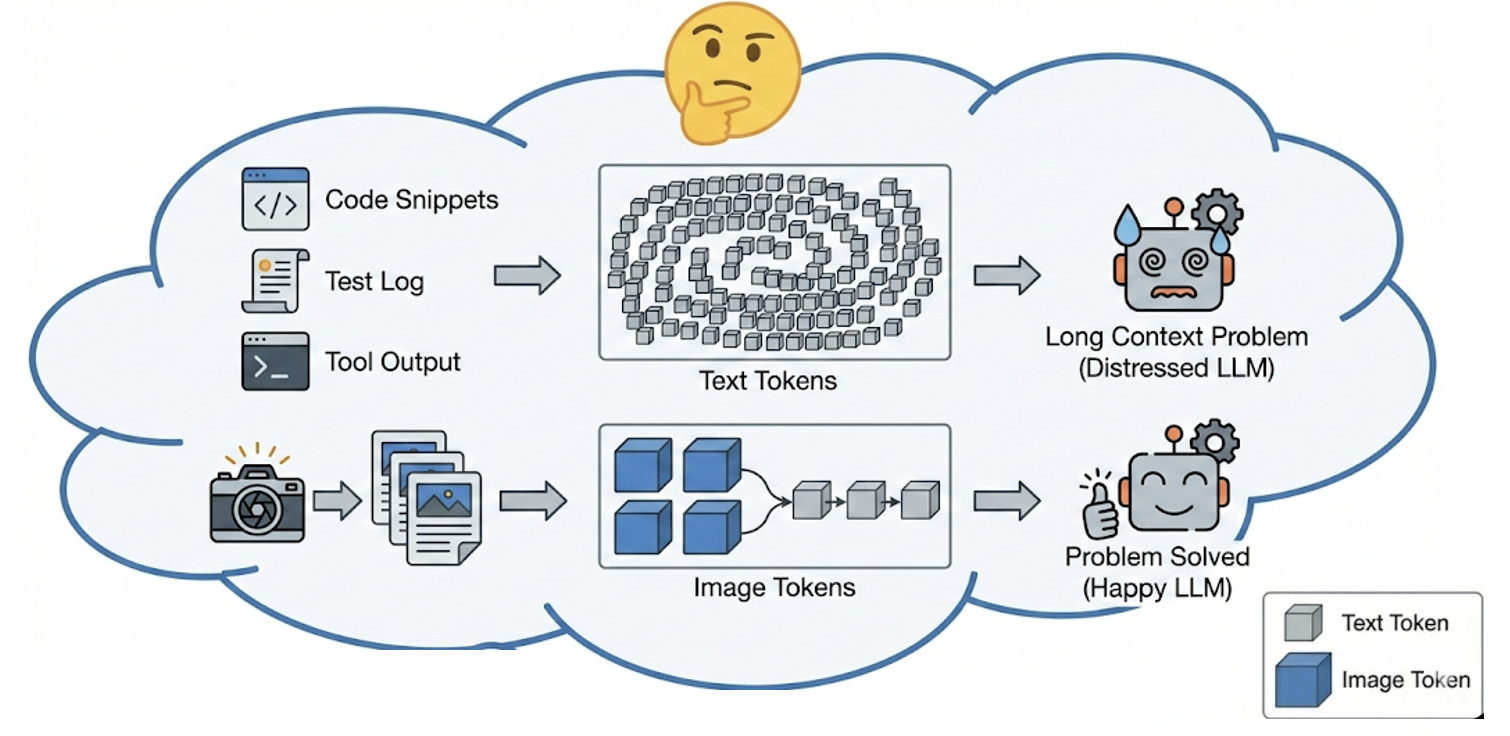
\includegraphics[width=\linewidth]{Sections/figures/overview.png}
  \caption{Overview of our main idea. Evaluating coding LLM on long context input: plain-text vs.\ ``OCR'' compression.}
  \vspace{-2em}
  \label{fig:overview}
\end{figure}


\para{Proposed Approach.}
As shown in Figure~\ref{fig:overview}, we evaluate optical compression as a drop-in replacement for text-based code context in an agentic coding pipeline. We build on mini-swe-agent \cite{yang2024sweagent} and implement an OpticalAgent that intercepts code-heavy tool outputs (identified by a simple heuristic) and renders them as monospace images before passing them to GPT-5-mini. The issue description and non-code outputs (error messages, directory listings, short search results) remain as text. This observation-level design ensures that the bulk of code the model reads, namely file contents accessed via file-reading commands, is presented as images.

\para{Experiments.}
We conducted a two-phase evaluation. First, a \emph{readability pilot study} swept rendering parameters (font sizes 8--20pt, page widths 100--140 characters) across six diverse Python code samples, establishing that GPT-5-mini achieves $\le$1.5\% character error rate and 100\% identifier recall at 12pt/120-character width. Second, we ran the full agentic pipeline on a 100-instance stratified subset of SWE-bench Verified, comparing the text baseline against the optical condition. We measured resolve rate, token usage, dollar cost, wall clock time, and behavioral differences.

\para{Results.}
We draw two main conclusions. First, \textbf{optical code input without any post-training is fully viable}: the vision-capable model reads and reasons about code from images as accurately as from text, achieving identical resolve rates (51/100 for both conditions), with 41 instances resolved by both and 10 unique to each. Second, \textbf{image tokens are currently more expensive than text tokens}: the optical agent consumes 29\% more input tokens and costs 1.9$\times$ more per instance (\$0.06 vs.\ \$0.03). Realizing the cost-saving potential of optical compression will likely require post-training to reduce the number of vision tokens per image, as explored by concurrent work such as DeepSeek-OCR \cite{wei2025deepseekocr}.

\para{Contributions.}
The main contributions of this work are:
\begin{itemize}[leftmargin=*]
  \item A readability pilot study establishing that GPT-5-mini can reliably read Python source code from rendered images (CER $\le$1.5\%, 100\% identifier recall), with an analysis of error patterns including the model's tendency to semantically rewrite regex rather than transcribe it.
  \item A controlled evaluation demonstrating that optical code input is a viable drop-in replacement for text in an agentic coding pipeline, achieving equivalent resolve rates (51\% vs.\ 51\%) on SWE-bench Verified without any post-training.
  \item An analysis showing that while feasible, optical encoding is currently more expensive per instance, suggesting that post-training (e.g., learned visual encoders) is needed to make optical compression cost-competitive.
\end{itemize}
